%\documentclass[preprint]{aastex} %double-column, single-spaced document:
\documentclass[iop,floatfix]{emulateapj} 

\usepackage{hyperref}
\usepackage{graphicx}
\usepackage{apjfonts}
\usepackage{enumerate}
\usepackage{amsmath,amssymb}
\usepackage{bm}
\usepackage[usenames,dvipsnames,svgnames,table]{xcolor} 
\usepackage[utf8]{inputenc}

%version-control tagging based off of github.com/bd-j/speccal
%%% This file is generated by Makefile.
\newcommand{\githash}{b3f5d1c}\newcommand{\gitdate}{2014-08-19}\newcommand{\gitauthor}{Ian Czekala}

\newcommand{\prob}{{\rm prob}}
\newcommand{\qN}{\{q_i\}_{i=1}^N}
\newcommand{\qM}{\{q_{im}\}_{i=1,m=0}^{N,M}}
\newcommand{\yN}{\{y_i\}_{i=1}^N}
\newcommand{\vt}{\vec{\theta}}
\newcommand{\vg}{\vt_{\star, {\rm grid}}}
\newcommand{\vpp}{\vt_{\star, {\rm post}}}
\newcommand{\vstar}{\vt_{\star}}
\newcommand{\finst}{f_{\lambda, {\rm inst}}}
\newcommand{\fsynth}{f_{\lambda, {\rm synth}}}
\newcommand{\vN}{\vt_{\rm N}}
\newcommand{\vc}{\vec{c}}
\newcommand{\fM}{ {\bm M}}
\newcommand{\fMi}{M_i}
\newcommand{\fD}{ {\bm D}}
\newcommand{\fDi}{D_i}
\newcommand{\fR}{ {\bm R}}
\newcommand{\dd}{\,{\rm d}}
\newcommand{\trans}{\mathsf{T}}
\newcommand{\Z}{[{\rm Fe}/{\rm H}]}
\newcommand{\A}{[\alpha/{\rm Fe}]}
\newcommand{\matern}{Mat\'{e}rn}

\newcommand{\todo}[1]{ \textcolor{Blue}{\\TODO: #1}}


%% Nomenclature guide
%%%%%%%%%%%%%%%%%%%%%
% * collections of synthetic spectra are generically called ``libraries.'' The term 
% ``grid'' is used when referring specifically to the spacing of spectral parameters
% in the library 

\shorttitle{Spectroscopic inference}
\shortauthors{Czekala et al.}

\begin{document}

\graphicspath{{figs/}}

\title{A Method for the spectroscopic inference of fundamental stellar parameters}
\author{\today{}\\
\medskip
Ian~Czekala\altaffilmark{1} et al.
%Author2\altaffilmark{2},
}

\altaffiltext{1}{Harvard-Smithsonian Center for Astrophysics, 60 Garden Street 
 MS 10, Cambridge, MA 02138}
%\altaffiltext{2}{Institution 2}
\email{iczekala@cfa.harvard.edu}

\section{Introduction}
\begin{itemize}
  \item Where our technique fits in the ecosystem of stellar methods.
  \item Applicable to any kind of spectrum (long-slit, echelle, infrared,
    flux-calibrated or not)
  \item Examples of fields where accurate and unbiased stellar parameters are
    crucial. Exoplanets. T Tauri stars.
\end{itemize}

\section{Method}
Typically, the stellar properties we most desire are effective temperature
 $T_{\rm eff}$, radius or surface gravity $\log g$, and metallicity $\Z$.
Several high-quality libraries of synthetic spectra now exist (PHOENIX, Kurucz,
 more being developed for GAIA) and are parameterized by these fundamental
 stellar parameters, which together, we call $\vg$. 
Synthetic libraries provide high-resolution spectra which span a range of $\vg$
 covering the main sequence of spectral types. The library is typically
 specified on a grid of equal spacing in $T_{\rm eff}$, $\log g$, and $\Z$.

In addition to these fundamental parameters, a star also has several observed
 properties that are a function of its kinematics, geometry, and location in our
 galaxy: projected rotational velocity $v \sin i$, line of sight velocity $v_z$,
 total extinction $A_V$, and solid angle $\Omega$. 
We call these secondary parameters $\vpp$, because we can model their effects
 on the synthetic spectra in a ``post-processing'' step by convolution with an
 appropriate kernel or multiplication with a smooth function. 
Together, we call $\vstar = \{\vg, \vpp\}$.

Using a synthetic stellar library as a backend and applying post-processing
 techniques, we attempt to forward-model the observed stellar spectra in order
 to determine the best-fit $\vstar$. 
Because properly sampled spectra have correlated pixels, we present a framework
 which self-consistently models these correlations. 

%\begin{table}[!htb]
%\begin{tabular}{ll}
%\hline
%\hline
%Symbol & Description\\
%\hline
%\hline
%$i$ & index specifying a pixel\\
%$\lambda_i$ & wavelength corresponding to a given pixel $i$\\
%$\vg$ & fundamental stellar parameters, $T_{\rm eff}, \log(g), \Z, \A$\\
%  & that parameterize a synthetic spectrum from the grid\\
%$\vpp$ & stellar parameters $v \sin i$, $v_z$, $A_V$, and $R^2/d^2$ that\\
%  & are applied during ``post processing'' of the synthetic spectrum\\
%$\vstar$ & $\{\vg,\vpp \}$\\
%$\finst(\lambda)$ & data spectrum\\
%$\fsynth(\lambda)$ & synthetic spectrum\\
%$c_0, c_1, \ldots$ & Chebyshev polynomial coefficients for residual flux calibration\\
%$\vN$ & the set of nuisance parameters composed of $\{c_0, c_1, \ldots, c_N\}$\\
%$\vt$ & the parameters $\{\vg, \vpp, \vN\}$ that completely describe a model spectrum\\
%$\fDi$ & data flux for a given pixel, $D(\lambda_i)$\\
%$\fD$ & data vector comprised of all $\fDi$, $i = \{0, \ldots, N\}$\\
%$\fMi$ & model flux for a given pixel, $M(\lambda_i | \vt)$\\
%$\fM$ & model vector comprised of all $\fMi$, $i = \{0, \ldots, N\}$\\
%$\sigma_i$ & Poisson noise for a given pixel $i$\\
%$R_i$ & residuals $\fDi - \fMi$\\
%$\fR$ & residual vector $\fD - \fM$\\
%$C$ & covariance matrix\\
%$k_{\rm global}$  & global covariance kernel\\
%$k_{\rm region}$  & regional covariance kernel\\
%\hline
%\end{tabular}
%\caption{Nomenclature used in this document}
%\label{tab:nomenclature}
%\end{table}

\begin{figure*}[!htb]
\begin{center}
  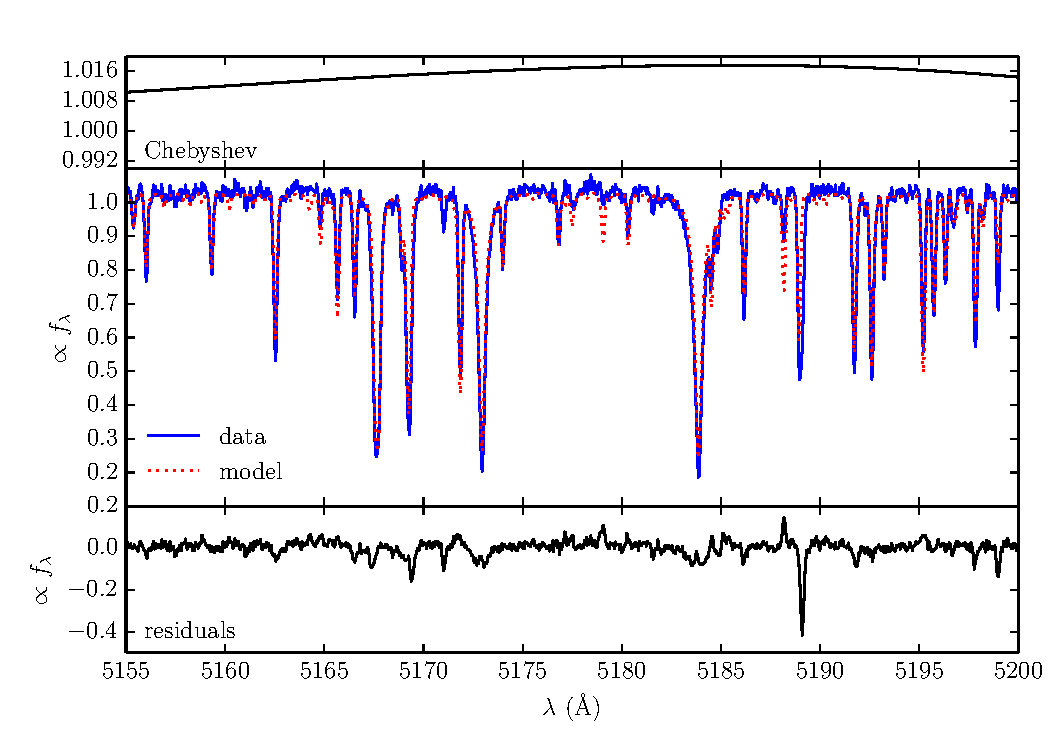
\includegraphics{figs/model_data.pdf}
  \caption{\textbf{Top}: Chebyshev polynomial which modifies the model spectrum
   to account for inaccuracies in the flux-calibration. 
  \textbf{Middle}: The data spectrum and model spectrum, after it has been
   interpolated, post-processed, and multiplied by the Chebyshev polynomial.
  \textbf{Bottom}: Residuals from the model fit. Note the large residual at
   $\lambda5189$\AA\ due to a missing opacity source from \ion{Ca}{1}. 
  \protect \todo{Model spectrum will be updated once I properly burn in the
   chain. Do these line styles look OK? I was going for something legible
   that might also print well in B/W}.}
\label{fig:model_data}
\end{center}
\end{figure*}

\subsection{Interpolation from synthetic spectral libraries}
Creating a new spectrum with a specific $\vg$ requires either synthesizing a
 new spectrum using radiative transfer codes or interpolating from nearby grid
 points in the library. 
Because it is computationally expensive to synthesize a spectrum at high
 resolution over a wide wavelength range, we choose to interpolate. 
Spline interpolation for spectra \citep{hus12}.
\todo{Implement band-limited interpolation from the synthetic grid using spline
 interpolation. Caution: As is, 100K/0.5 logg spacing in $\vg$ may not be
 Nyquist sampling.}
\todo{Investigate a ``Bayesian Emulator'' for using Gaussian processes for
 interpolating from a simulation grid.}

\subsection{Post-processing synthetic spectra to match the data}
Libraries of synthetic spectra are generally computed at high resolution ($R
 \geq $100,000), sampled with many pixels per resolution element, and do not
 include any rotational broadening or account for any instrumental effects. 
In order to transform a raw synthetic spectrum interpolated from the grid into
 one that matches the spectrum of a real star, we must post-process the spectrum
 to account for these secondary effects. 
The projected rotational velocity of the star, parameterized by $v \sin i$,
 broadens spectral line profiles and is mathematically described by convolution
 with a kernel $g_{v \sin i}(\lambda)$.  
UV, optical, and infrared spectra are acquired using a spectrograph which
 disperses light onto a CCD, defining a specific resolution and sampling rate
 for the spectrum. 
Because the resolution of the spectrograph and spacing of the pixels are
 different from the synthetic spectral library, we must convolve the raw
 spectrum with the line spread function (LSF) of the instrument $g_{\rm
 LSF}(\lambda)$ and resample to the exact pixels of the CCD. In wavelength
 space, the $v \sin i$ and LSF operations are represented by the convolution of
 the synthetic spectrum with these two kernels
\begin{equation}
  \finst(\lambda) = g_{v \sin i}(\lambda) \otimes g_{\rm LSF}(\lambda) 
   \otimes \fsynth(\lambda)
  \label{eqn:convolution}
\end{equation}
Using the convolution theorem, we can rewrite these operations as
 multiplications in Fourier space 
\begin{equation}
  F_{\lambda, {\rm inst}}(s) = G_{\rm LSF}(s) G_{v \sin i}(s) F_{\lambda, 
    {\rm synth}}(s)
\end{equation}
 where $G \leftrightarrow g$ and $F \leftrightarrow f$ are Fourier transform
 pairs. 
In order to use the fast Fourier transform (FFT) to execute these
 operations using discrete samples of the synthetic spectrum $\fsynth$, we must
 first resample $\fsynth$ so that it is on a uniform grid. 
In the case of a spectrum, the natural uniform grid is one that is equally
 sampled in velocity space, such there is an equal velocity shift $\Delta v$
 between pixels. This results in a wavelength grid that is linearly sampled in
 the logarithm of wavelength. 
Therefore, the Fourier coordinate $s$ is the number of cycles per sampling
 interval, having units of inverse velocity $[{\rm s}/{\rm km}]$. 
Next, we multiply the Fourier transform of the synthetic spectrum by the
 Fourier transforms of the rotational velocity and line spread function kernels.
Lastly, we do an inverse FFT to transform the modified spectrum $F_{\lambda,
 {\rm inst}}$ back to wavelength space, where it is sampled at the wavelength
 locations of the pixels in the detector ($\finst$). 
When resampling the spectrum, we are careful to ensure band-limited
 interpolation using splines in order to prevent introducing non-physical high
 frequency structure into the spectrum.

Finally we apply corrections for interstellar extinction and Doppler shift.
Interstellar extinction attenuates the spectrum by an amount $A_\lambda$, which
is wavelength-dependent. 
We use the (name here) dust-extinction model, which is parameterized by
 extinction in the $V$ photometric band, $A_V$. 
We correct for a radial velocity difference $v_z$ between the star and the
 earth by Doppler shifting the model spectrum. 
\todo{Doppler shifting the wavelengths could be implemented as a phase-shift in
 Fourier space, but it's pretty fast as-is.}

\todo{We might try implementing the convolution in wavelength space, rather
 than the FFT. 
This would allow the LSF to change with wavelength.\\} 
Pixel width effects are not important as long as the LSF of the instrument is
 adequately sampled ($\gtrsim 3$ pixels across the LSF). 
If our spectrum were not properly sampled, we would need to additionally
 convolve with a boxcar the width of the pixels.

\begin{figure*}[!htb]
\begin{center}
  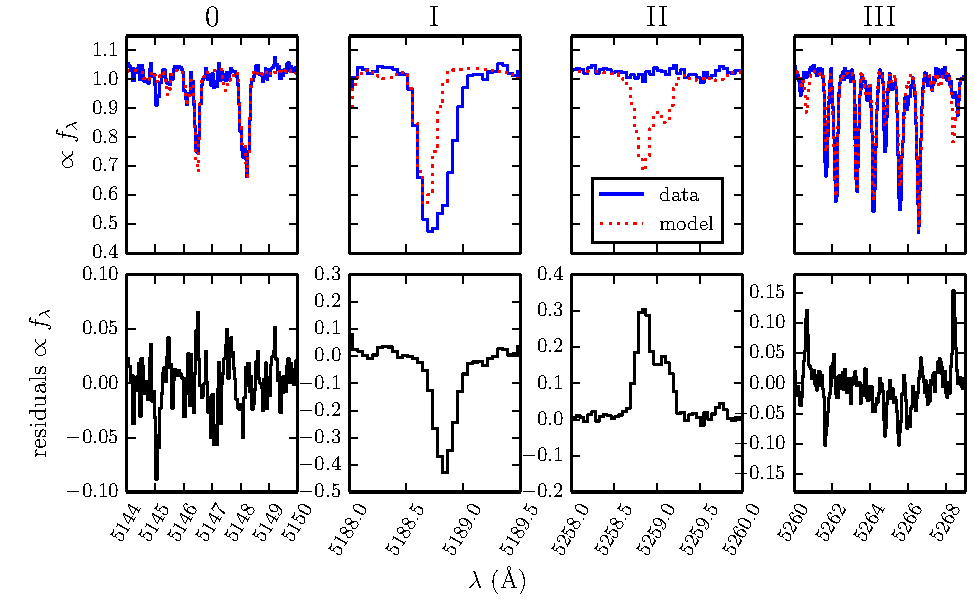
\includegraphics[width=0.9\textwidth]{figs/badlines.pdf}
  \caption{The variety of residual behaviour, depending on the quality of model
    fit. 
    From left to right: \textbf{Class 0} covariance results from slight
     model mismatch, and correlates nearby residuals. 
    \textbf{Class I}: A missing absorption line in the model leaves a large,
     highly correlated patch of negative residuals. 
    \textbf{Class II}: An extraneous line in the model leaves a large, highly
     correlated patch of positive residual.  
    \textbf{Class III}: If lines are present in the model but of the wrong
     strength, many correlated residuals of moderate amplitude will result. 
    The difficulty with class III lines is that for any specific line, there might
     exist a $\vstar$ that will fit the line, but there does not exist a
     $\vstar$ that will properly fit \emph{all} the lines.}
\label{fig:badlines}
\end{center}
\end{figure*}

Due to small imperfections in the flux-calibration of the data spectrum, there
 may be broad regions of the spectrum which are offset from the true continuum
 level by a slight amount. 
A traditional approach to address this problem is to normalize both the data
 and the spectrum to the continuum level before comparison. 
While this may work well for hotter stars with well-defined continuua, for
 cooler stars with large molecular features, normalization may introduce
 artificial features into the spectrum when the pseudo-continuum is incorrectly
 placed. 
Instead, we choose to multiply the model spectrum by a low-order Chebyshev
 polynomial that is normalized to unity. 
The coefficients of the polynomial, $c_0, c_1, \ldots$, will be free-parameters
 in our model that we will solve for. 
If the behavior of the spectrograph is characterized by observations of
 spectrophotometric standards, then we can put priors on the coefficients that
 will prevent overfitting of the polynomials. 
For an example of a typical spectrum, and Chebyshev polynomial, see
 Figure~\ref{fig:model_data}.

With more uncertainty, the polynomial multiplication can also be used as a
 substitute for flux-calibration since the sensitivity function of an instrument
 is usually a smooth function with wavelength. 
When spectra are not flux calibrated, there is greater uncertainty about the
 properties of the spectrograph and wider priors must be used on the Chebyshev
 coefficients. 
In this case, the polynomial might destroy broad-scale information present in
 the spectrum by fitting it out, something that would be avoided with more
 accurate priors provided by the flux calibration for the model.

\subsection{Likelihood function}
To evaluate which parameters of the model $\fM$ fit the data set $\fD$ best we
 use a standard multidimensional Gaussian likelihood function which allows for
 covariance between data points. 
If the vector of residuals is 
\begin{equation}
  \fR(\vstar) = \fD - \fM(\vstar)
\end{equation}
 with a length of $N$ data points, then the likelihood function is
\begin{equation}
  p(\fD | \vstar) = \frac{1}{\sqrt{(2 \pi)^N \det(C)}} \exp\left ( -\frac{1}{2}
   \fR^T C^{-1} \fR \right ) 
\end{equation}
 and the log-likelihood function is
\begin{equation}
  \ln[p(\vstar)] = -\frac{1}{2} \fR^T C^{-1} \fR - \frac{1}{2} \ln \det C  
   - \frac{N}{2} \ln 2 \pi 
  \label{eqn:lnprob}
\end{equation}
$C$ is the covariance matrix which describes the covariance between pixels in
 the spectrum. 
For independent noise with noise per pixel $\sigma_i$, this matrix is diagonal
\begin{equation}
  C = 
  \begin{bmatrix}
    \sigma_0^2 & 0  & \cdots & 0\\
    0 & \sigma_1^2 & \cdots & 0\\
    \vdots  &   & \ddots  & \vdots \\
    0 & 0 & \cdots & \sigma_N^2\\
  \end{bmatrix}
  \label{eqn:covariance_diagonal}
\end{equation}
with $\sigma_{ij} = 0$ everywhere and equation~\ref{eqn:lnprob} reduces to the
 familiar $\chi^2$ form of a sum over the square of the residuals, weighted by
 the inverse variance of each data point
\begin{equation}
  \ln[p(\vstar)] \propto - \frac{1}{2} \chi^2 = - \frac{1}{2} \sum_i
   \frac{R_i^2}{\sigma_i^2}
\end{equation}

However, residuals from a spectroscopic fit are often correlated due to
 \todo{DUE TO WHAT, exactly?? I'm confused. 
Wait for response from Tom Loredo}. 
Additionally, systematic errors in the synthetic spectra (such as incorrect
 line strengths) will result in regions of highly correlated residuals. 
Properly accounting for correlations in the residuals requires that we use a
 covariance matrix with off-diagonal terms $\sigma_{ij}$ and a likelihood
 function (Equation~\ref{eqn:lnprob}) which uses a matrix product instead of a
 sum over independent pixels.

We seek to understand and parameterize two types of covariance structure in our
 model, exemplified in Figure~\ref{fig:badlines}: the large scale but generally
 mild global covariance structure that results from [still to be finalized
 cause], and a regional covariance structure that is localized to areas where
 spectral line mismatch results in small patches of highly correlated residuals. 
Ignoring the complexity of spectroscopic residuals will bias the estimates of
 the model parameters $\vt$. 

As a simple analogy, consider the fit of a straight line to a dataset. 
If the noise in the dataset is correlated, then adjacent data points might be
 offset from the linear trend in the same direction by a similar amount. 
If the covariant structure of the noise is ignored, a simple $\chi^2$ will
 treat these correlated offsets as part of the linear trend, which will result
 in a biased determination of the slope and intercept of the line, typically
 with uncertainties that are too small.

\subsection{Parameterizing the covariance structure}
We parameterize the covariance structure using covariance kernels, which sets
 the covariance between two pixels $\lambda_i$ and $\lambda_j$. 
This behavior is analogous to the two-point correlation function used in
 cosmology, where the distance between two galaxies is used instead of
 wavelength.

\paragraph{Global covariance structure}
A global covariance structure may result from a slight mismatch in the
 continuum or mild mismatch of spectral lines like that shown as class 0 in
 Figure~\ref{fig:badlines}. 
To account for this structure, which is generally mild and typically exists
 across only a few pixels, we use a \emph{stationary} covariance kernel, which
 satisfies the property that the degree of correlation only depends on the
 distance between the two pixels $r$. 
Functions like this are also called \emph{radial basis functions}. 
For spectra, we map $r$ to the velocity difference between two pixels
\begin{equation}
  r(\lambda_i, \lambda_j) = \Delta v = \frac{c}{2} \left | \frac{\lambda_i 
   - \lambda_j}{ \lambda_i + \lambda_j} \right |
\end{equation}
We choose the \matern\ $3/2$ kernel because\ldots
\todo{Explore difference between using \matern\ kernel and squared exponential
 kernel. 
Why \matern\ and why Hann? 
Because they are the vanilla covariance functions that are tried and tested in
 the machine learning communities.}
\begin{equation}
  k_{\nu = 3/2}(r, a, l) = a \left(1 + \frac{\sqrt{3} r}{l} \right ) \exp 
   \left (- \frac{\sqrt{3} r}{l} \right )
\end{equation}
In order to keep the covariance matrix sparse for computational efficiency, we
 taper for compact support using a Hann window
\begin{equation}
  w(r, r_0) = \frac{1}{2} + \frac{1}{2} \cos \left( \frac{\pi r}{r_0} \right) 
\end{equation}
for a global covariance kernel of 
\begin{equation}
  k_{\rm global} (r, a, l, r_0) = w(r, r_0) k_{\nu = 3/2}(r, a, l) 
  \label{eqn:global}
\end{equation}
We add this covariance kernel to the independent variance already present along
 the matrix diagonal
\begin{equation}
  k(\lambda_i, \lambda_j) = k_{\rm global}(r, a, l, r_0) + \delta_{ij} \sigma_{ij}^2
\end{equation}
where $\delta_{ij}$ is the Kroenecker delta function.

\begin{figure*}[!htb]
\begin{center}
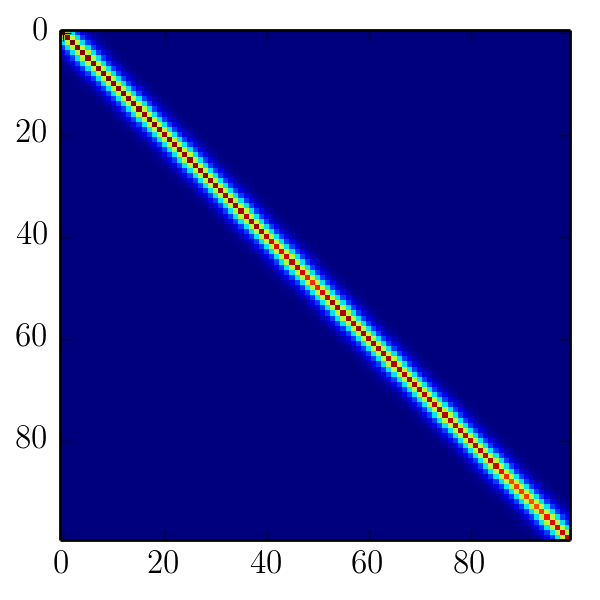
\includegraphics[width=0.4\textwidth]{figs/matern_matrix.png}
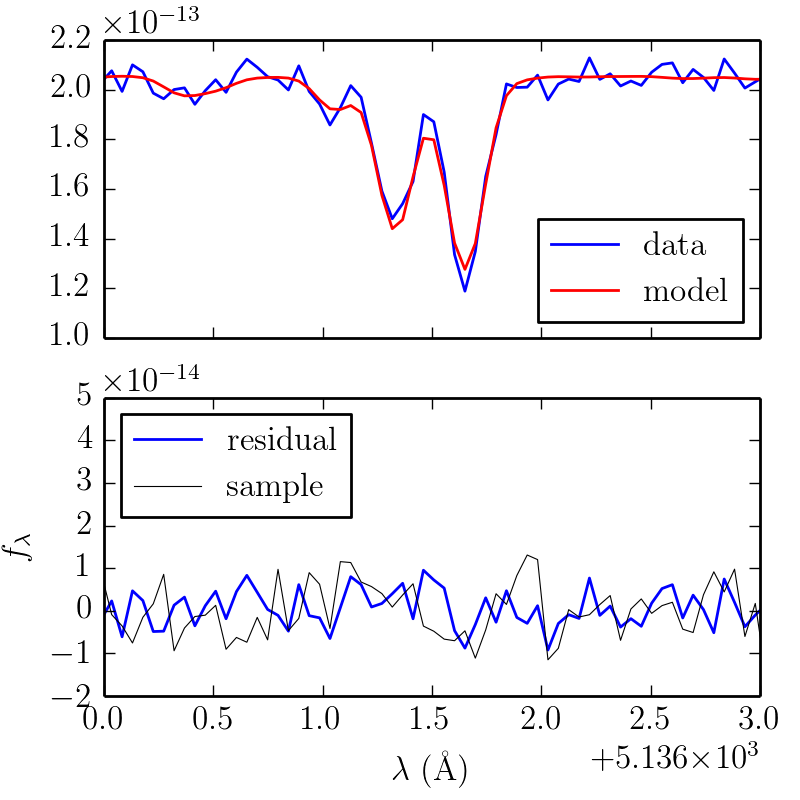
\includegraphics[width=0.4\textwidth]{figs/matern_draw.png}
\caption{\textbf{Left} a covariance matrix generated with the \matern\ kernel
 and typical parameters for our dataset.  
 \textbf{Right} general spectroscopic residuals near a stellar continuum
  overlaid with a sample draw using the covariance matrix, showing that the two
  look similar in structure and amplitude. 
  \protect \todo{Prettify these figures. Consistent labelling. Change
  color stretch so Matrix zeros are white.}}
\label{fig:matern}
\end{center}
\end{figure*}

To visualize what the covariance matrix $C$ might look like when parameterized
 by Equation~\ref{eqn:global}, see the left panel of Figure~\ref{fig:matern}. 
To explore the relationship between the parameters of the covariance kernel and
 the properties of the noise, first consider simulating uncorrelated random
 Gaussian noise by drawing many independent samples from a Gaussian. 
This same uncorrelated noise could also be represented as a single draw from a
 $N$-dimensional Gaussian with a diagonal covariance matrix, like in
 Equation~\ref{eqn:covariance_diagonal}. 
If instead of a diagonal covariance matrix, we were to draw samples from a
 non-trivial covariance matrix like the one in the left panel of
 Figure~\ref{fig:matern}, then we will see correlated noise like in the right
 panel. 
\todo{Do you think examples like Figure~\ref{fig:matern} are helpful or a waste
 of space?}


\paragraph{Specific line covariance} For the large and highly correlated
 residuals that result from class I, II, and III line errors, we use a
 \emph{non-stationary} covariance kernel, which means that the covariance
 explicitly depends on $\lambda_i$ and $\lambda_j$.
\todo{Explain how we come up with this kernel, which is the covariance
 resulting from a Gaussian function.}
\begin{equation}
  k_{\rm G}(\lambda_i, \lambda_j | a, \lambda_\mu, \sigma) = 
   \frac{a^2}{2 \pi \sigma} \exp \left ( - \frac{r^2(\lambda_i, \lambda_\mu) 
    + r^2(\lambda_j, \lambda_\mu)}{2 \sigma^2}\right )
\end{equation}
The squared exponential kernel is
\todo{Why do we use the squared exponential and not \matern?}
\begin{equation}
  k_{ \rm exp}(r, h) = \exp \left ( \frac{- r^2 }{2 h^2} \right )
\end{equation}
$h$ is a bandwidth. 
If $h$ is small, then there will be high-frequency structure. If $h$ is large,
 then only low-frequency structure will remain. 
We also use the Hann window to taper the kernel for compact support
\begin{equation}
  k(\lambda_i, \lambda_j | h, a, \mu, \sigma, r_0) = 
   w(r, r_0)\; k_{ \rm exp}(r, h) \; 
   k_{\rm G}(\lambda_i, \lambda_j | a, \mu, \sigma)
\end{equation}

\todo{Similar paragraph about visualizing the covariance matrix, drawing
  samples. References to Figure~\ref{fig:region}.}

\begin{figure*}[!htb]
\begin{center}
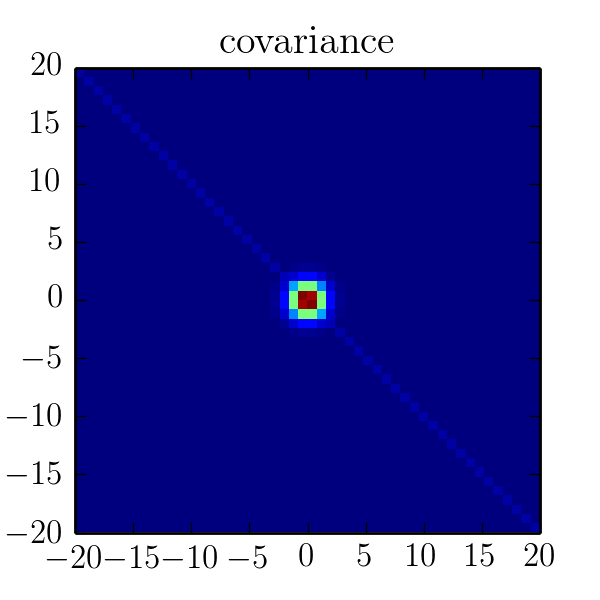
\includegraphics[width=0.4\textwidth]{figs/matrix_region_covariance.png}
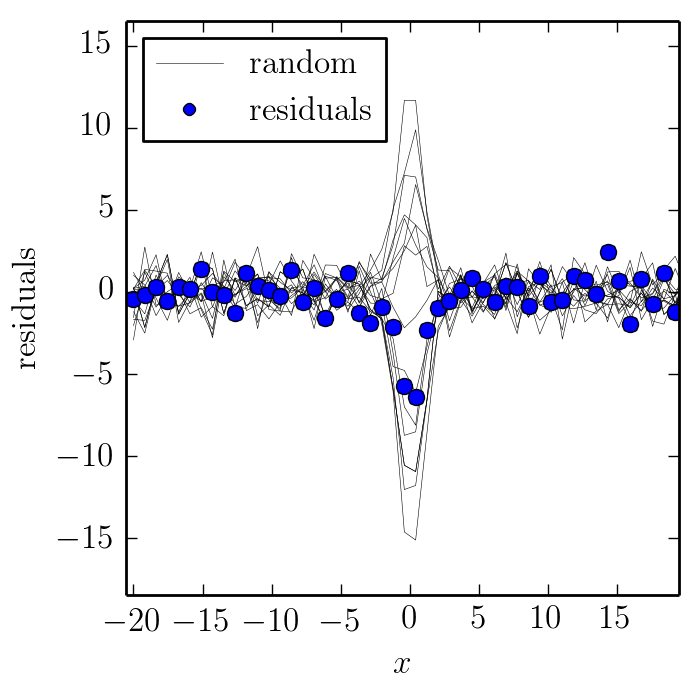
\includegraphics[width=0.4\textwidth]{figs/random_draw.png}
\caption{\textbf{Left} a covariance matrix generated with the region kernel.
\textbf{Right} general spectroscopic residuals near a mismatched stellar line
 overlaid with a sample draw using the covariance matrix, showing that the two
 look similar in structure and amplitude. 
\protect \todo{Similar improvements to
  Figure~\ref{fig:matern}.}}
\label{fig:region}
\end{center}
\end{figure*}

\begin{itemize}
  \item non-stationary kernel localizes increased variance to a specific
    spectral line
  \item better than just masking out the region, since these contain info
  \item there will be many sets of regions ($\sim$1-4\% of all lines might be
    covered by a region)
  \item there can be hyperparameters describing the \emph{population} of
    regions in a hierarchical model (mostly width, amplitude).
\end{itemize}

Covariance kernel parameters are parameters in our model that we explicitly
 sample for. 

The benefit mainly comes from simply modelling these systematic residuals to
 begin with, since a model with covariance is far more likely than forcing the
 fit, and far more justified than masking regions which do not fit.

\todo{Show how the kernel can accounts for complicated M dwarf structure where
 there is large, messy mismatch.}

\subsection{Exploring the posterior}
Markov Chain Monte Carlo
\todo{Given this is 2014 and not 2010, how much do you think I need to explain?}

\subsection{Applications}
Learnt covariance structure can be used to correct the models.

\section{Tests}
\todo{Which tests to show?}

This version of the paper was generated
 from a git repository available at \url{http://github.com/iancze/StellarSpectra/}
 with git hash \texttt{\githash\,(\gitdate)}.

\bibliography{stellarspectra}
\bibliographystyle{hapj}
\end{document}
